\chapter{INTRODUCTION}
\label{chap:intro}
In the era of Google glass, %people wants everything in front of them to be explicable.
everybody wants everything, including video to be explained.  Just like in football, one would like to obtain the highlights of a match in terms of statistics, such as duration of ball control by respective team and more.  While in the sphere of surveillance, detecting multiple simultaneous events is very crucial.  All these tasks are broadly categorized as an application of video event recognition. 

\par A video event is defined as \textit{a fact or process of doing things to attain a goal}.  Video events may be short like a player kicking the ball or long as player scoring a goal.  It is noticed that most of the annotated events available are short events, also long events can be modelled as sequence of short events.  Only short events are considered in this work.  While the subject of event can be any physical objects like human, ball etc.
\par The problem of video event recognition is generally framed as prediction of video event from given set of labelled internet videos, where the label specifies the events that occurs within video.  But most of the datasets available are in weakly labelled settings, i.e they do not have spatio-temporal segmentation indicating coordinates and time points where and which event occurs.  Therefore the particular problem can bifurcated as localization and prediction problem.  The localization aspect of the problem is the task of locating the event within the video %and further build train of frame corresponding to the event
and then building a sequence of frames.  The train of frames correspond to the spatio temporal volume (STV) and are used by models for the prediction.
\par Even though the recognition appears to be simple there are quite a lot of challenges.  Most of the challenges observed are centred around the source of the video like dynamic background, moving camera, low lighting and more.  Another challenging aspect of this problem is to deal with large intra-category variations for achieving satisfactory classification on wide scale of videos.
\par Generally, such problems are tackled in the following manner : local feature extraction, feature aggregation, finally a classifier (such as SVM) to distinguish among the visual classes of interest.  But these approaches suffer from one major challenge, namely, the choice of feature that best represents video.  In last few years, deep neural network has revolutionized the machine learning field and has edified a new approach for training.  In the case of deep neural network, it accepts raw input rather than the processed features and generates (bottleneck) features in process of prediction. 
\par Convolutional neural network (CNN), a deep learning method has shown remarkable success for the visual recognition task as it takes advantages of the spatial structure of images/videos.  It was also observed resistant to translational variances and also supported several regularization tricks for address the large intra-category variances.  Therefore the CNN's are considered for  the event recognition problem.

\clearpage
\section{Outline of the Work}
A novel solution to the problem of video localization and recognition has been proposed. In the approach the input video is given to background subtraction to measure variation in pixel intensity in continuous frames.  Also the saliency measure is obtained for train of frames that capture the regions in the frame that are quite distinct in the frame.  Both the measure are fused to obtain a new score termed visual attention score (VAS) that can capture the motion as well as the contrast in given frame. 
\par CNN is being considered for event recognition which expects fixed size raw image/video as input. Therefore a spatio temporal volume (STV) corresponding to video event are extracted by smoothening the VAS to obtain bounding box that is being tracked along the sequence of frames.  Figure \ref{fig:outline} depicts the outline of the proposed solution to the event recognition problem.
\begin{figure}[htpb]
   \begin{center}
	    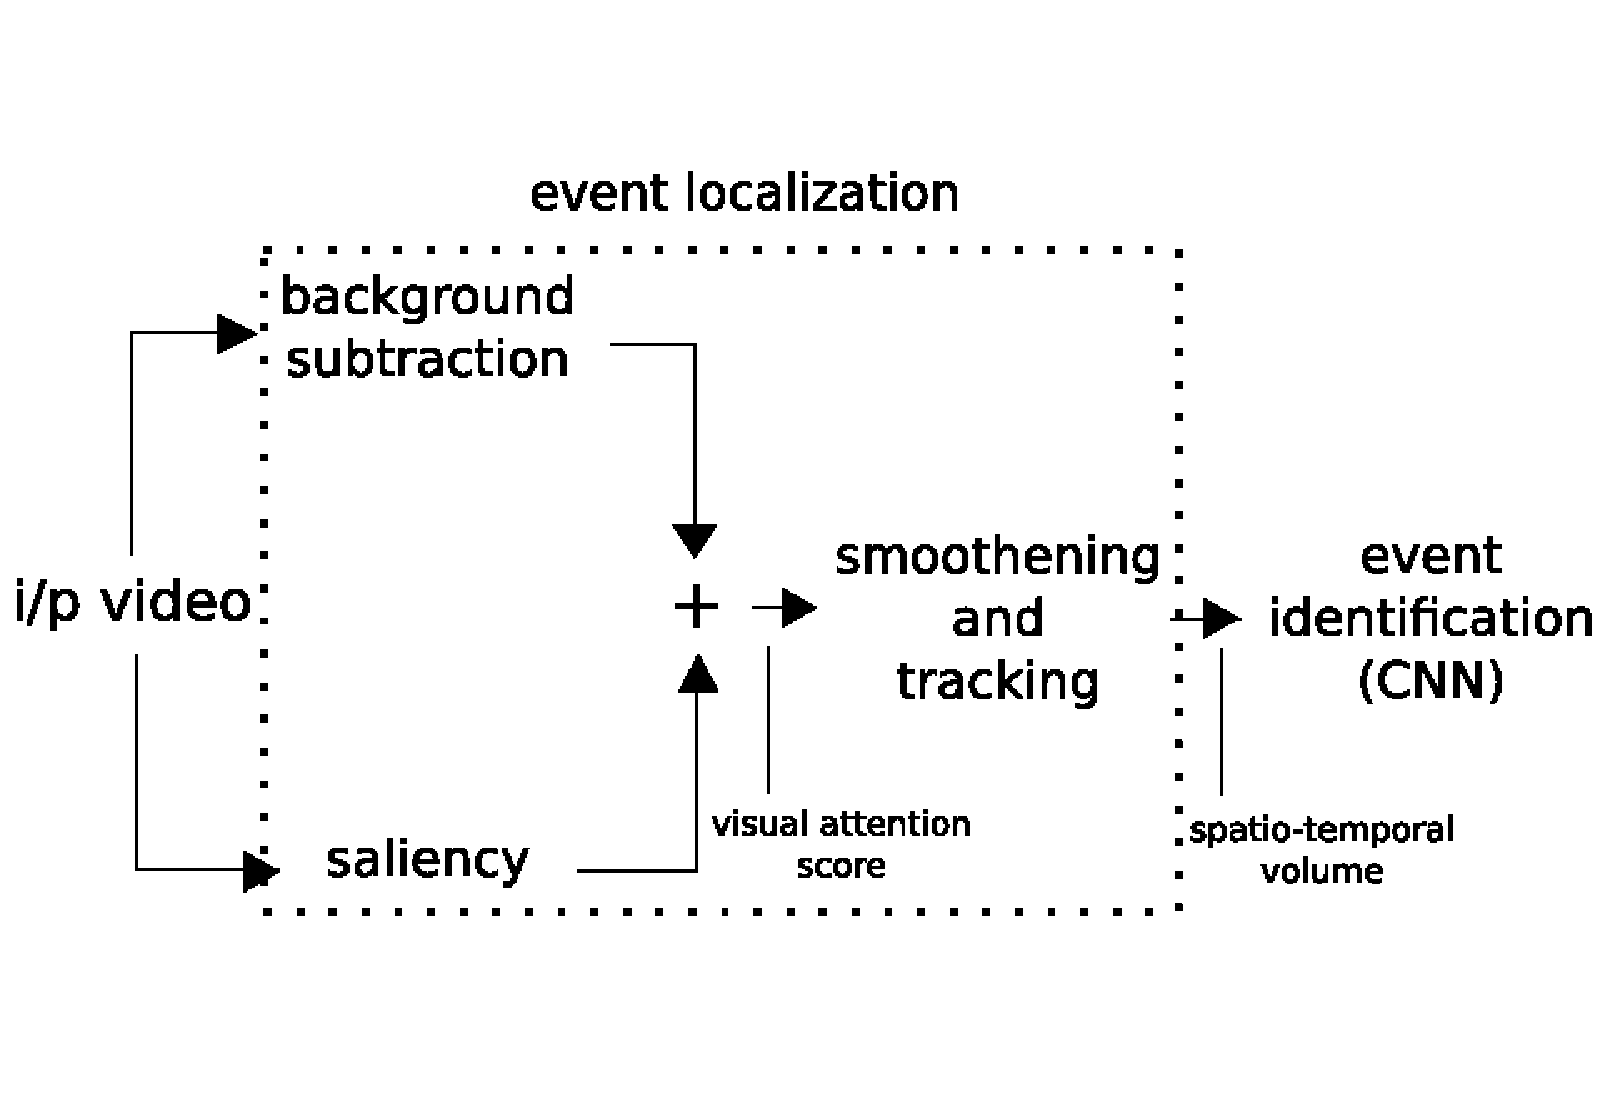
\includegraphics[width=0.95\textwidth]{snaps/outline.eps}     
     \caption {Proposed solution for video event recognition}
   \label{fig:outline}
   \end{center}
 \end{figure}
 
\section{Major Contribution}
\begin{itemize}
	\item{Built a indigenous deep neural network toolkit providing an ease to configure for different neural network models.}
	\item{Proposed a novel approach to obtain visual attention score by fusing the background subtraction and saliency measure.}
	\item{Suggested different ways for performing temporal smoothening over the visual attention score by considering a temporal context.}
	\item{Devised algorithm for extracting spatio temporal volume from the smoothed scores.}
\end{itemize}

\section{Organization of thesis}
\par Chapter \ref{chap:eventrec} includes discussion about the existing techniques used for event recognition and the home-grown implementation of neural network.  While in chapter \ref{chap:eventLo} steps for extracting spatio-temporal volume by fusing background subtraction and saliency measure is being elaborated.  The experiments for the event recognition and the justification for choosing the appropriate techniques for the ultimate model are chalked in chapter \ref{chap:exp}.  The future scope and the summary of the entire work can be seen in chapter \ref{chap:concl}.